\documentclass{beamer}
\usepackage[spanish]{babel}
\usepackage[latin1]{inputenc}
\usepackage{multicol} % indice en 2 columnas
\usepackage{graphics, graphicx}
\usepackage{listings}             % Incluye el paquete listings
\usepackage{adjustbox}



\usetheme{Warsaw}
\usecolortheme{seahorse}
\useoutertheme{shadow}
\useinnertheme{rectangles}
\graphicspath{ {/home/emanuel/Tesis/Tesis/Documentos/img/} }

\setbeamertemplate{navigation symbols}{} % quitar simbolitos


\title[]{Optimizaci\'on del c\'omputo para la resoluci\'on del problema de una y dos part\'iculas en un pozo de potencial usando B-splines}
\author[]{Emanuel Lupi}

\institute[]
{
  Universidad Nacional de C\'ordoba\\
  FaMAF
}
\date{26 de Marzo de 2018}

\begin{document}

\frame{\titlepage}




\begin{frame}
  \frametitle{Introducci\'on}
  \begin{block}{Ecuaci\'on de Sch\"odringer}
    \begin{displaymath}
        E\psi(r) = \left[\frac{-\hbar^2}{2\mu} \nabla^2 + V(r)\right]\psi(r)
    \end{displaymath}
  \end{block}

  \begin{block}{Ecuaci\'on de Schr\"odinger independiente del tiempo}
      \begin{displaymath}\label{ec_schrodinger}
        \mathcal{H} |\psi_n(\vec{r})\rangle = E_n |\psi_n(\vec{r})\rangle\,,
      \end{displaymath}
  \end{block}

  \begin{block}{Ecuaci\'on radial}
    \begin{displaymath}
        -\frac{\hbar^2}{2m} \frac{1}{r^2}\frac{d}{dr}\left(r^2\frac{dR_n(r)}{dr}\right) 
        + \frac{\hbar^2\,l(l+1)}{2m\,r^2}\,R_n(r) + V(r)\,R_n(r) = E_n\,R_n(r)\,.
    \end{displaymath}
  \end{block}
\end{frame}


\begin{frame}
  \frametitle{Discretizaci\'on}
   
  \begin{block}{Ec reducida}
  \begin{displaymath}
    \phi_n(r) = r\,R_n(r)\,,
  \end{displaymath} 
  \begin{displaymath}
    -\frac{1}{2} \frac{d^2 \phi_n}{dr^2} + \frac{l(l+1)}{2\,r^2} \phi_n(r) + V(r)\,\phi_n(r) = E_n\,\phi_n(r)\,,
  \end{displaymath} 
  \end{block}
  \begin{displaymath}\label{combinacion_lineal}
      \phi_n(r)=\sum_{i=1}^{N}\alpha_i\,\varphi_i(r) = \sum_{j=i-k+1}^{i}\alpha_j\varphi_j(r)\ para\ r\ \in\ [t_i, t_{i+1}]\,,
  \end{displaymath}

  \begin{figure}[!tbp]
    \centering
    \includegraphics[width=0.5\textwidth]{uniform-b-splines.eps}
  \end{figure}
\end{frame}


\begin{frame}
    \frametitle{Ecuaciones Lineales}
    \begin{displaymath}\label{ec_auval}
    H_l \vec{\alpha} = E\,S\,\vec{\alpha}\,,
    \end{displaymath}

    \noindent 
    para $E$ y $\lbrace\alpha_i\rbrace_1^N$, d\'onde

    \begin{align}\label{elemento_matriz}
    (H_l)_{ij} &= -\frac{1}{2} \int_0^{r_{max}} \varphi_i(r) \frac{d^2}{dr^2}\varphi_j(r) \,dr \nonumber
               + \frac{l(l+1)}{2}\int_0^{r_{max}} \frac{\varphi_i(r) \,\varphi_j(r)}{r^2} \,dr \\
               & + \int_0^{r_{max}} \varphi_i(r)\,V(r)\,\varphi_j(r)\, dr \\
    (S)_{ij} &= \int_0^{r_{max}} \varphi_i(r)\,\varphi_j(r)\,dr \label{solapamiento}
    \end{align}
\end{frame}

\begin{frame}
  \frametitle{Extendiendo a dos Part\'iculas}

  \begin{displaymath}\label{hamiltoniano2p}
    \mathcal{H}_{2p} = \mathcal{H}_{1p}^{(1)} + \mathcal{H}_{1p}^{(2)} + U(\vec{r}_1,\vec{r}_2)\,,
  \end{displaymath}
  \begin{displaymath}\label{eq:scho-2p}
    \mathcal{H}_{2p} \psi_n(\vec{r}_1,\vec{r}_2) = E_n^{2p} \psi_n(\vec{r}_1,\vec{r}_2)\,,
  \end{displaymath}
  \begin{displaymath}\label{base-2p}
    \chi_{i,j}(r_1,r_2) = \left\lbrace \begin{array}{ccc}
                        \varphi_i(r_1)\,\varphi_j(r_2) & \mbox{si} & i=j \\
                        \frac{\varphi_i(r_1)\,\varphi_j(r_2)+\varphi_i(r_2)\,\varphi_j(r_1)}{\sqrt{2}} & \mbox{si} & i\neq j
                        \end{array} \right.\,,
  \end{displaymath}
  \begin{displaymath}\label{base-2p-2}
    \hat{\chi}_{i,j}(r_1,r_2) = \varphi_i(r_1)\,\varphi_j(r_2)\,,
  \end{displaymath}
  \begin{displaymath}\label{mat-hamiltoniano-2p}
    \begin{split}
    H_{i,i';j,j'} &= \langle \hat{\chi}_{i,j} |\mathcal{H}_{2p}|\hat{\chi}_{i',j'}\rangle \\
                  &= (H_l)_{i,i'}\,S_{j,j'} + S_{i,i'}\,(H_l)_{j,j'} + U_{i,i';j,j'}\,,
    \end{split}
  \end{displaymath}

  \begin{displaymath}\label{matriz_interaccion}
    \begin{split}
      U_{i,i';j,j'} &= \langle \chi_{i,j} |U(r_1,r_2)|\chi_{i',j'}\rangle \\
                    &=  \int_0^{r_{max}} \left(\int_0^{r_{max}} \varphi_i(r_1)\, \varphi_j(r_2)\,
                    U(r_1,r_2)\, \varphi_{i'}(r_1)\, \varphi_{j'}(r_2)\, dr_2\right)\, dr_1\,.
    \end{split}
  \end{displaymath}
\end{frame}

\begin{frame}
  \frametitle{El proceso}
  \textit{El m\'etodo que se optimiz\'o tiene las siguientes partes}
  \begin{itemize}
    \item {Armar el sistema
      \begin{itemize}
        \item El c\'alculo de las abscisas y pesos de la Cuadratura de Gauss-Legendre.
        \item C\'alculo de las matrices $H$ y $S$
        \item C\'alculo de la matriz U de interacci\'un. (En el sistema de 2 part\'iculas solamente)
        \item C\'alculo del sistema de dos part\'iculas $H_{2p}$ y $S_{2p}$. (En el sistema de 2 part\'iculas solamente)
      \end{itemize}}
    \item {Resolver el sistema
  \begin{itemize}
    \item Usar alg\'un resolvedor de autovalores y autovectores con $H$ y $S$.
  \end{itemize}
  }
  \end{itemize}
\end{frame}


\begin{frame}
  \frametitle{Matrices dispersas}
  \begin{figure}[!tbp]
    \centering
    \includegraphics[width=0.7\linewidth]{smat.eps}
    \caption{Matriz S.}
  \end{figure}
\end{frame}



\begin{frame}
  \frametitle{Matrices dispersas}
  \begin{figure}[!tbp]
    \centering
    \begin{minipage}[b]{0.4\textwidth}
      \includegraphics[width=\textwidth]{hsim20.eps}
      \caption{$H_{2p}$ L=20.}
    \end{minipage}
    \hfill
    \begin{minipage}[b]{0.5\textwidth}
        \includegraphics[width=\textwidth]{hsim50.eps}
        \caption{$H_{2p}$ L=50.}
    \end{minipage}
  \end{figure}

\end{frame}

\begin{frame}
  \frametitle{Matrices dispersas}
  \begin{figure}[!tbp]
    \centering
    \begin{minipage}[b]{0.5\textwidth}
      \includegraphics[width=\textwidth]{vef.eps}
      \caption{Matriz U.}
    \end{minipage}
    \hfill
    \begin{minipage}[b]{0.4\textwidth}
        \includegraphics[width=\textwidth]{matricita_vef.eps}
        \caption{Bloque de U.}
    \end{minipage}
  \end{figure}
\end{frame}


\lstset{language=C, breaklines=true, basicstyle=\footnotesize}


\defverbatim[colored]\lstI{
\begin{lstlisting}[
language=C++,
basicstyle=\ttfamily,
keywordstyle=\color{red},
basicstyle=\tiny,
tabsize=2,
showspaces=false]
for(unsigned int m = 1; m<KORD; ++m)
  for(unsigned int n = m; n<KORD; ++n)
    for(unsigned int j = 0; j<INT_G; ++j) {
      double bm = 0, bn = 0;
      rr = x[idx(k[i], j)];
      bm = bder(rr, m, KORD);
      bn = bder(rr, n, KORD);
      ...
    }
\end{lstlisting}
}

\defverbatim[colored]\lstII{
\begin{lstlisting}[
language=C++,
basicstyle=\ttfamily,
keywordstyle=\color{red},
basicstyle=\tiny,
tabsize=2,
showspaces=false]
for(unsigned int j = 0; j<INT_G; ++j) {
  rr = x[idx(k[i], j)];

  for(unsigned int m = 1; m<KORD; ++m) 
    bders[m] = bder(rr, m, KORD);

  for(unsigned int m = 1; m<KORD; ++m) 
    for(unsigned int n = m; n<KORD; ++n) {
      double  bm = bders[m],
              bn = bders[n];
      ...
    }
}
\end{lstlisting}
}

\begin{frame}{Refactorizaci\'on de C\'odigo}{}
  \textit{Antes}
  \lstI
  \textit{Despues}
  \lstII
\end{frame}

\begin{frame}{Rec\'alculo de funciones simples}{}
  \begin{displaymath}
    T(i) = \left\lbrace \begin{array}{ccc}
                        R_{min} & \mbox{si} & i < KORD \\ \\
                        R_{min} + dr * i  & \mbox{si} & KORD \leq i < KORD + L_{INT}\\ \\
                        R_{min} + dr *\\ (KORD + L_{INT} - 1) & \mbox{si} & KORD + L_{INT} \leq i
                        \end{array} \right.\,
  \end{displaymath}
\end{frame}

\begin{frame}{Escalado de Gauss Legendre}{}
  \begin{block}{Cuadratura de Gauss Legendre}
    \begin{displaymath}
      \int_{-1}^{1} f(x) dx \approx \sum_{i=1}^{n}w_if(x_i)
    \end{displaymath}
    \begin{displaymath}
      \int_{a}^{b} f(x) dx = \frac{b-a}{2} \sum_{i=1}^{n}w_if(\frac{b-a}{2}x_i + \frac{a+b}{2})
    \end{displaymath}
  \end{block}
\end{frame}


\begin{frame}{Optimizaci\'on GPU}{}
  \begin{displaymath}
  kernel_1 \left\lbrace \begin{array}{ccc}
    f_{j,j'}(r_1) &=& \int_0^{r_1} \varphi_j(r_2)\,U(r_1,r_2)\,\varphi_{j'}(r_2)\,dr_2 \,, \\
    g_{j,j'}(r_1) &=& \int_{r_1}^{r_{max}} \varphi_j(r_2)\,U(r_1,r_2)\,\varphi_{j'}(r_2)\,dr_2 \,,
  \end{array} \right.\,
  \end{displaymath}

  \begin{displaymath}
    U_{i,i';j,j'} = \int_0^{r_{max}} \varphi_i(r_1)\,f_{j,j'}(r_1)\,\varphi_{i'}(r_1)\,dr_1 + 
                    \int_0^{r_{max}} \varphi_i(r_1)\,g_{j,j'}(r_1)\,\varphi_{i'}(r_1)\,dr_1\,.
  \end{displaymath}

  \begin{displaymath}
    kernel_2 \left\lbrace \begin{array}{ccc}
    U_{i,i';j,j'} &=& \int_0^{r_{max}} \varphi_i(r_1)\,(f_{j,j'}(r_1) + g_{j,j'}(r_1))\,\varphi_{i'}(r_1)\,dr_1
    \end{array} \right.\,
  \end{displaymath}

\end{frame}

\begin{frame}{Otras optimizaciones}{}
  Como tenemos que $S_{ij} = S_{ji}$ solo se calcula la mitad superior
  Alojar las matrices del sistema en el espacio de variables globales
\end{frame}



\begin{frame}{Resultados una part\'icula tiempo}{}
  \begin{figure}[!tbp]
    \includegraphics[width=1\linewidth]{unaparticula.eps}
    \caption{Resultados Una particula en tiempo}
  \end{figure}
\end{frame}

\begin{frame}{Resultados una part\'icula tiempo}{}
\begin{table}[H]
\begin{center}

\small
\begin{tabular}{ |c|c|c|c| }
  \hline
  $L_{INT}$ & Tiempo No Optimizado & Tiempo Optimizado & Speed Up \\
  \hline
  40 & 0.185 & 0.008 & 21.944\\
  50 & 0.225 & 0.009 & 25.051\\
  80 & 0.370 & 0.014 & 26.874\\
  100 & 0.457 & 0.015 & 30.524\\
  150 & 0.682 & 0.022 & 30.535\\
  200 & 0.918 & 0.026 & 34.652\\
  250 & 1.177 & 0.037 & 32.090\\
  300 & 1.368 & 0.042 & 32.908\\
  350 & 1.632 & 0.050 & 32.498\\
  400 & 1.832 & 0.050 & 36.648\\
  450 & 2.124 & 0.064 & 33.020\\
  500 & 2.335 & 0.071 & 33.087\\
  550 & 2.554 & 0.077 & 33.038\\
  600 & 2.778 & 0.080 & 34.703\\
  650 & 3.067 & 0.091 & 33.782\\
  \hline
\end{tabular}
\caption{Speed Up No Optimizado vs Optimizado una part\'icula}
\label{table:speedup1par}
\end{center}
\end{table}
\end{frame}

\begin{frame}{Resultados una part\'icula memoria}{}
\begin{figure}[!tbp]
    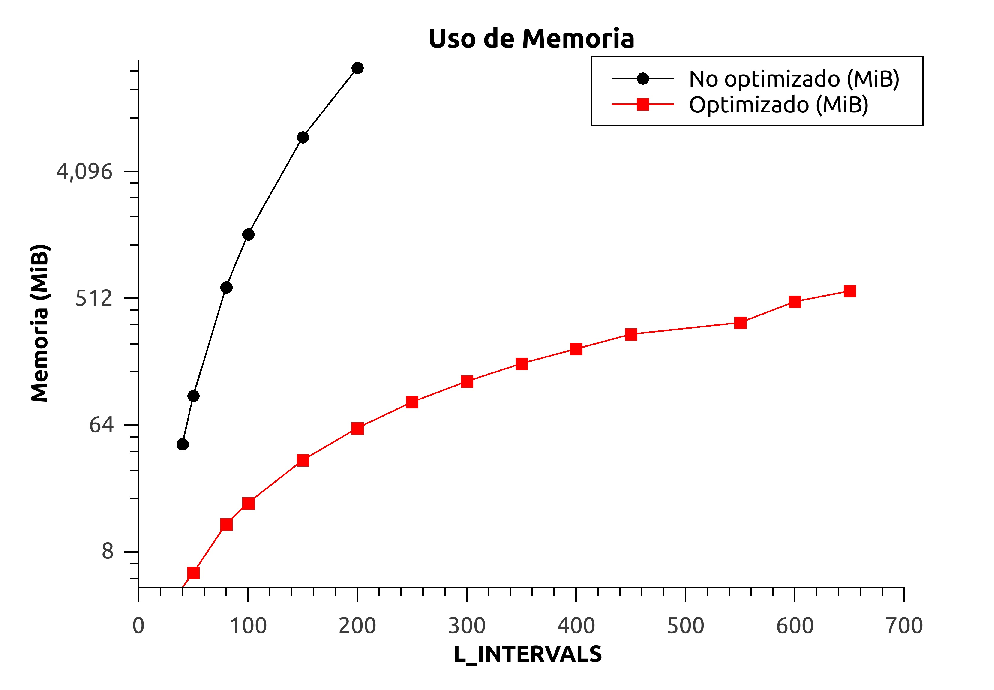
\includegraphics[width=1\linewidth]{memoria.eps}
    \caption{Resultados Una particula en memoria}
  \end{figure}
\end{frame}

\begin{frame}{Resultados dos part\'iculas}{}
  \begin{figure}[h]
  \renewcommand\figurename{Gr\'agico}
  \begin{center}
    \leavevmode

    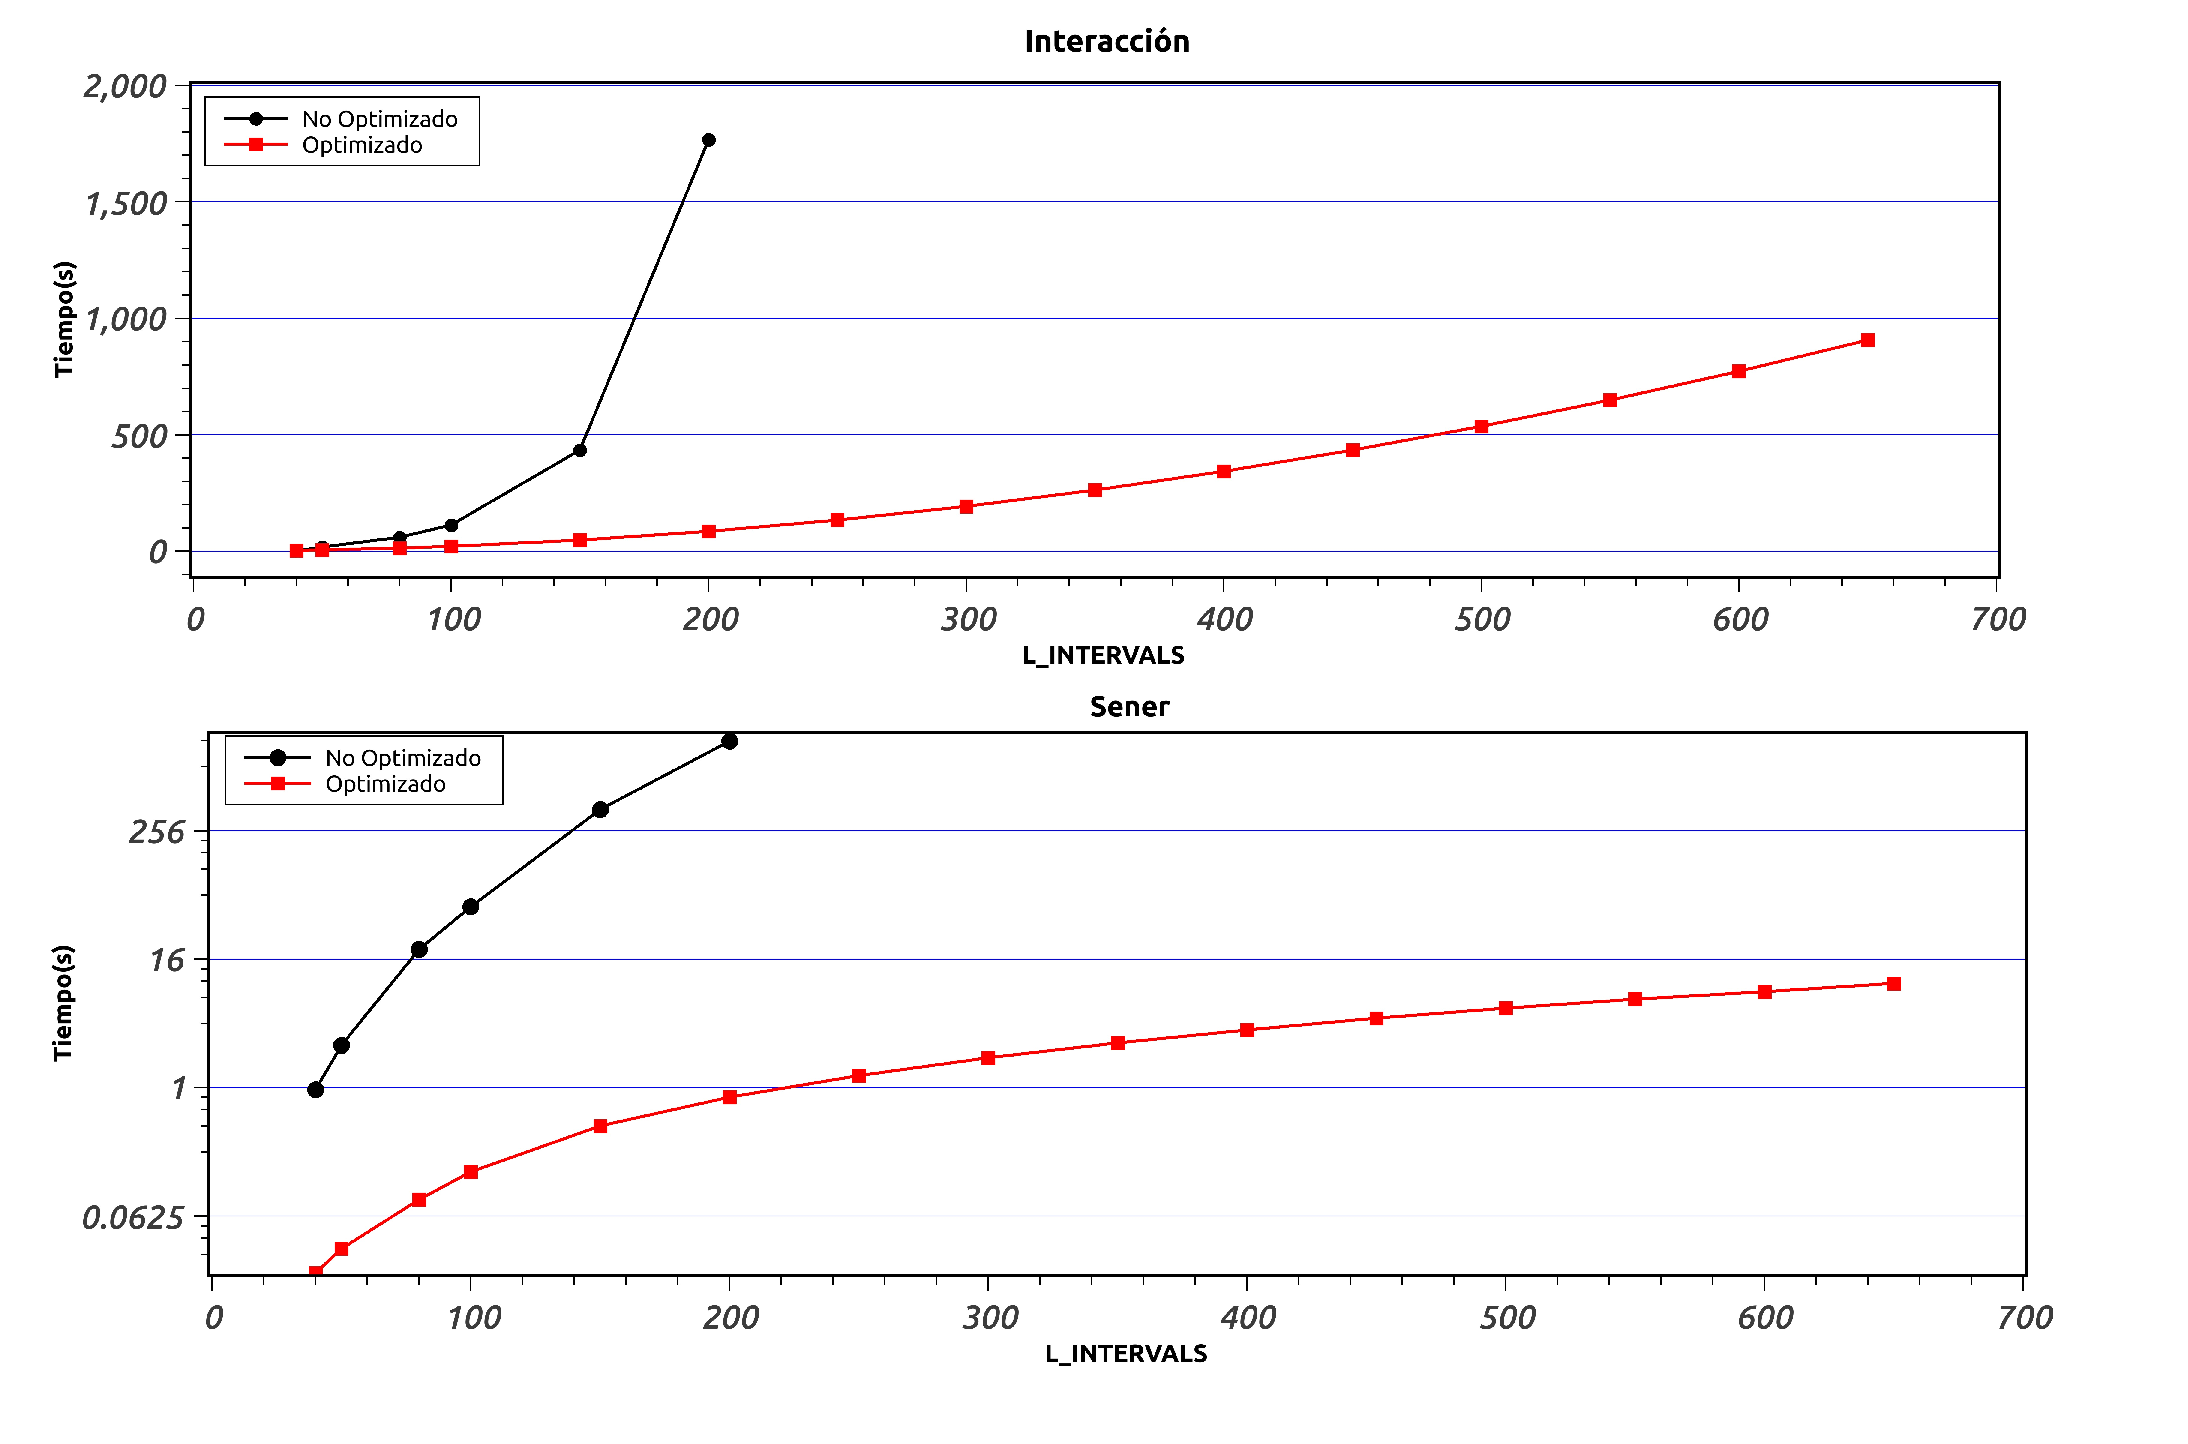
\includegraphics[width=0.9\linewidth]{optimizado2.eps}

  \end{center}
\end{figure}
\end{frame}

\begin{frame}{Resultados dos part\'iculas}{}
  \begin{table}[H]
  \begin{center}

  \begin{adjustbox}{max width=\textwidth}
  \begin{tabular}{ |c|c|c|c|c|c|c| }
    \hline
    $L_{INT}$ & Interacci\'on  & Sener    & Interacci\'on & Speed Up & Sener      & Speed Up \\
              &                &          & Optimizado    &          & Optimizado & \\
    \hline
    40  & 0.63    & 0.05    & 3.35    & 0.19  & 0.02  & 2.81 \\
    50  & 18.41   & 0.14    & 5.26    & 3.50  & 0.03  & 4.58 \\
    80  & 60.11   & 1.51    & 13.55   & 4.44  & 0.09  & 16.89 \\
    100 & 112.81  & 3.80    & 21.20   & 5.32  & 0.16  & 23.35 \\
    150 & 434.46  & 19.69   & 48.13   & 9.03  & 0.44  & 44.97 \\
    200 & 1766.32 & 63.13   & 85.69   & 20.61 & 0.81  & 77.48 \\
    \hline
  \end{tabular}
  \end{adjustbox}

  \end{center}
  \end{table}
\end{frame}

\begin{frame}{GPU}{}
  \begin{figure}[h]
    \renewcommand\figurename{Gr\'agico}
    \begin{center}
      \leavevmode
   
      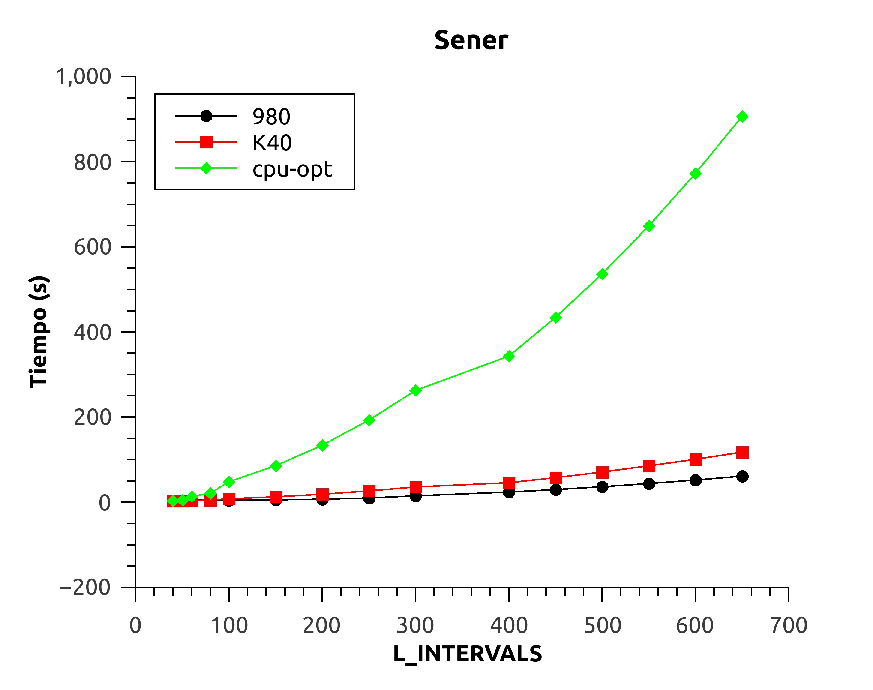
\includegraphics[width=1\linewidth]{cpu_vs_gpu.eps}

      \caption{Comparaci\'on entre CPU y GPU}

      \label{graph:cpu_vs_gpu}
    \end{center}
  \end{figure}
\end{frame}

\begin{frame}{GPU}{}
\begin{table}[h]
\begin{center}

\small
\begin{tabular}{ |c|c|c|c|c|c| }
  \hline
  $L_{INT}$ & Tiempo CPU &   Tiempo   & Speed Up & Tiempo K40 & Speed Up \\
               &            &   GTX980   &  GTX980  &            &    K40\\
  \hline
  80 & 13.553 & 5.494 & 2.467 & 4.410 & 3.073\\
  100 & 21.201 & 4.288 & 4.944 & 5.164 & 4.106\\
  150 & 48.133 & 4.809 & 10.009 & 8.552 & 5.628\\
  200 & 85.695 & 6.169 & 13.891 & 13.550 & 6.325\\
  250 & 133.899 & 7.936 & 16.871 & 20.167 & 6.639\\
  300 & 192.871 & 11.364 & 16.972 & 28.515 & 6.764\\
  350 & 262.632 & 16.948 & 15.497 & 38.551 & 6.813\\
  400 & 343.160 & 27.332 & 12.555 & 49.341 & 6.955\\
  450 & 434.191 & 34.075 & 12.742 & 62.108 & 6.991\\
  500 & 536.205 & 41.716 & 12.854 & 76.332 & 7.025\\
  550 & 648.931 & 50.266 & 12.910 & 92.064 & 7.049\\
  600 & 772.392 & 59.990 & 12.875 & 108.469 & 7.121\\
  650 & 906.392 & 70.547 & 12.848 & 126.974 & 7.138\\
  \hline
\end{tabular}
\caption{Speed Up No Optimizado vs Optimizado dos part\'iculas}
\label{table:speedupgpu}
\end{center}
\end{table}
\end{frame}

\begin{frame}{Conclusiones}{}
  \textit{Lista de prioridades a la hora de optimizar}
  \begin{itemize}
    \item Identificar que funciones son las mas pesadas.
    \item Conocer el flujo u operaciones del programa.
    \item Estudiar las estructuras de las variables involucradas.
    \item Elejir las estructuras de datos m\'as adecuadas.
    \item Optimizar el flujo u operaciones del programa.
      \begin{itemize}
        \item Adaptar el c\'odigo a las nuevas estructuras
        \item Modificar el flujo del c\'odigo.
        \item Vectorizar (si se da el caso)
      \end{itemize}
    \item Escalar horizontalmente.
  \end{itemize}
\end{frame}

\begin{frame}{?`Preguntas?}{}
\end{frame}

\end{document}